\chapter{Background}
\label{ch:background}

In this chapter the background on both the planning and optimization aspect of this thesis is presented.
The concepts and techniques discussed in this chapter are employed in the framework we propose in \autoref{ch:methodology} with the aim of optimizing for a probabilistic model that can be used to obtain plans which maximize the performance of a system that is in need of automated control.

First of all, in \autoref{sec:decision-theoretic-planning}, the chapter discusses how \acrfull{acr:dtp} deals with the central problem of planning under uncertainty using probabilistic models of a system under consideration.
In this thesis we put our attention to modeling \acrshort{acr:dtp} problems as \acrfullpl{acr:mdp} and accordingly discuss the existing algorithmic techniques for obtaining plans for automated \acrfull{acr:sdm}.
We employ these ideas in the framework we propose in \autoref{ch:methodology} to compute optimal plans from the \acrshort{acr:mdp} models learned from data, to assess the value of different models.

Then, in \autoref{sec:bayesian-optimization}, the chapter elaborates upon a method known as \acrfull{acr:bo}, which is used to automate the process of optimizing the parameters of an unknown objective while minimizing the number of function evaluations.
This method is particularly suited for the optimization task dealt with in the framework proposed in \autoref{ch:methodology}, where the parameters of model learning algorithms are adjusted so to yield maximum performance in a system's execution.
That is, in our framework we assess the value of different \acrshort{acr:mdp} models by performing expensive simulations, which is why we would like to minimize the number of these simulations.
Therefore, in this section we describe how the \acrshort{acr:bo} framework achieves this and present some of its applications to related \acrshort{acr:sdm} problems.


\section{Decision-Theoretic Planning}
\label{sec:decision-theoretic-planning}

% Introduction on what is Decision-Theoretic Planning
Automated \acrfull{acr:sdm} comprises the central problem of planning under uncertainty. 
\acrfull{acr:dtp} is concerned with the design of plans or \textit{policies} for settings in which uncertainty exists about the effects of actions, where the decision maker or \textit{agent} has incomplete information about the environment and its initial conditions, and where trade-offs need to be made between potentially conflicting objectives to determine an optimal course of action.
This section gives an introduction to the type of problems faced in \acrshort{acr:dtp} and explains how specialized probabilistic models can be used to solve these problems efficiently.
First of all, in \autoref{sec:problem-formulation} the goal of \acrshort{acr:dtp} and how the problems that are considered are generally approached are discussed.
Subsequently, \autoref{sec:system-representation} gives an overview of the probabilistic models that are used to make the structure of problems in \acrshort{acr:dtp} explicit.
Then, \autoref{sec:learning-markov-models} discusses the algorithms that enable us to learn these models from a dataset describing the dynamics of the system under consideration.
Finally, in \autoref{sec:planning} some of the most common algorithmic planning techniques are discussed, which either learn a plan directly or through interaction.

\subsection{General Problem Formulation}
\label{sec:problem-formulation}
% Formulation of what kind of planning problems are considered in Decision-Theoretic Planning

The class of problems that are considered in \acrlong{acr:dtp} are those that require optimal stochastic control through the actions of decision maker(s), referred to as \textit{agent(s)}, in systems whose dynamics can be modeled as \textit{stochastic processes} \cite{Boutilier1999}.
The agent(s) in these systems sequentially need to choose from a set of actions that influence the system's behavior, consequently making the system switch from one state to another.
In these settings the system's current state and the agent's choice of action determines the probability distribution over the states the system might reach next.
In addition, the agent(s) might be uncertain about the system's current state, implying the need to infer from observations and making decisions based on probabilistic estimates of the system's state.

Typically the problems under consideration involve certain objectives to be achieved (e.g., tasks to be fulfilled) or properties to be satisfied (e.g., avoiding certain system states). 
Therefore, the agent should decide on an optimal plan or \textit{policy} which makes it most likely for the system to reach its targets, while minimizing the risk of producing undesirable states and the accompanied costs of the policy.
To find such a policy for \acrlong{acr:sdm} problems, a typical approach is to first setup a probabilistic model of the system and then apply a \acrshort{acr:dtp} algorithm on this model.
This probabilistic model comprises a system representation which defines the state space in terms of a set of multi-valued features, the set of actions the agent may select together with the associated uncertainty defined by transition probabilities, and a goal specification or performance metric typically expressed by means of a reward structure.

Overall \acrshort{acr:dtp} aims to devise planning algorithms for planning under uncertainty, a problem that is addressed in numerous different fields of research such as AI planning and control theory.
In particular difficulties arise when planning techniques are applied to determine courses of action for real-world settings, such as motion or path planning in robotics which both involve the possibility of action failures and disturbances caused by exogenous events.

\subsection{System Representations: Markov Models}
\label{sec:system-representation}
% Definitions of Markov Models relevant as probabilistic models for planning under uncertainty

As the class of problems considered in \acrshort{acr:dtp} tend to present considerable structure, there exist various proposed solutions for planning under uncertainty that apply model-based approaches.
This type of decision-theoretic planner uses a stochastic model of the environment in which the agent operates, which compasses the uncertainty that is associated with the agent's actions, observations and the exogenous events that might occur.
Typically the uncertainty is modeled by establishing a \textit{state space} for the system accompanied by a set of possible \textit{transitions} between the states that might be induced with a certain probability by an agent executing \textit{actions}.
The most common types of stochastic models that are used in \acrshort{acr:dtp} are called \textit{Markov Models} (sometimes also referred to as \textit{Markovian Models}), which has been motivated by their success in other fields such as speech recognition \cite{baker1992large, gales2008application, rabiner1989tutorial} and \acrfull{acr:rl} techniques \cite{kaelbling1996reinforcement, Brafman2002}.
A Markov Model is a stochastic model in which the future states only depend on a limited number of prior observations. In fact, mostly processes or systems are modeled by Markov Models that satisfy the \textit{Markov Property}, which means that the state transitions are independent of any previous states or agent actions.

In the remainder of this section the most common types of discrete-state Markov Models are discussed, starting from the fundamental models known as \textit{Markov Chains} and their extension known as \textit{\acrfullpl{acr:hmm}}.
These fundamental models however only describe the evolution of a system and do not allow for stochastic control.
Therefore, this is followed by a discussion of the discrete-state Markov Models known as \textit{\acrfullpl{acr:mdp}} and their extension known as \textit{\acrfullpl{acr:pomdp}}, which add the possibility of influencing the behavior of the system through sequential decisions.

%In the remainder of this section the most common types of discrete-state Markov Models are discussed one by one, starting from the fundamental models known as \textit{Markov Chains} in \autoref{subsec:markov-chains}, followed by their extension of \textit{\acrfullpl{acr:hmm}} in \autoref{subsec:hidden-markov-models}.
%This again is followed by a discussion of the discrete-state Markov Models most relevant in \acrshort{acr:dtp}, being \textit{\acrfullpl{acr:mdp}} in \autoref{subsec:mdps} and their extension of \textit{\acrfullpl{acr:pomdp}} in \autoref{subsec:pomdps}.
%Finally in \autoref{subsec:other-markov-models} other related state space models are briefly discussed.

\newpage

\subsubsection{Markov Chains}
\label{sec:markov-chains}
% Markov Chains: States and Transitions

The evolution of system or processes can be viewed as so-called \textit{time-series}, in which a set of datapoints can be ordered using an underlying physical dimension, typically time \cite{barberBRML2012}.
Formally, time-series can be defined as a series $x_{a:b}$ of datapoints, with $x_{a:b} \equiv x_a, x_{a+1}, \ldots, x_b$.
By means of these time-series, probabilistic models can be devised for real-world systems or processes, by introducing the notion of \textit{states} as a description of the system at a particular point in time or \textit{stage}.

On the basis of the class of Markov Models lies the simplifying assumption that each state is only dependent on a limited number of previous states.
Under this assumption a \textit{Markov Chain} (or \textit{Markov Process}) can be defined as a model of a series $q_{1:T}$ of transitions between states $q_i$ drawn from a state space $\mathcal{S} = \{s_1,\ldots,s_n\}$. The initial state $q_1$ of a Markov Chain typically is either fixed or drawn from $\mathcal{S}$ using a probability distribution over initial states.
For the states or variables of a Markov Chain, the earlier mentioned assumption implies the following conditional independence to hold:
\begin{equation}
p(q_t \vert q_1,\ldots,q_{t-1}) = p(q_t \vert q_{t - L}, \ldots, q_{t-1})
\end{equation}
where $L$ is the so-called \textit{order} of the Markov Chain.
% See summary barberBRML2012

\begin{figure}[t!]
	\captionsetup[subfigure]{justification=centering}
	\centering
	\subcaptionbox{First-order Markov Chain.\label{fig:markov-chains-first-order}}{\begin{tikzpicture}[->,>=stealth',auto,node distance=2cm]
		\tikzstyle{every state}=[fill=white,draw=black,text=black,scale=1,double]	% thick
		\node[state] (s1) {$q_1$};
		\node[state] (s2) [right of=s1] {$q_2$};
		\node[state] (s3) [right of=s2] {$q_3$};
		\coordinate (con) at (0,2);
		\path
		(s1)
		edge node {} (s2)
		(s2)
		edge node {} (s3)
		(s3);
		\draw [->, dashed, shorten >=0pt] (s3) to[right] node[auto] {} ++(1.3,0)
		;
		\end{tikzpicture}} \quad
	\subcaptionbox{Second-order Markov Chain.\label{fig:markov-chains-second-order}}{\begin{tikzpicture}[->,>=stealth',auto,node distance=2cm]
		\tikzstyle{every state}=[fill=white,draw=black,text=black,scale=1,double]	% thick
		\node[state] (s1) {$q_1$};
		\node[state] (s2) [right of=s1] {$q_2$};
		\node[state] (s3) [right of=s2] {$q_3$};
		\node[state] (s4) [right of=s3] {$q_4$};
		\path
		(s1)
		edge node {} (s2)
		(s2)
		edge node {} (s3)
		(s1)
		edge [bend left] node {} (s3)
		(s3)
		edge node {} (s4)
		(s2)
		edge [bend left] node {} (s4)
		;
		\draw [->, dashed, shorten >=0pt] (s4) to[right] node[auto] {} ++(1.3,0)
		;
		\end{tikzpicture}}
	\caption{Graphical representation of Markov Chains of different order.}
	\label{fig:markov-chains}
\end{figure}

As depicted in \autoref{fig:markov-chains}, Markov Chains of different order can be defined. \autoref{fig:markov-chains-first-order} exemplifying a first-order Markov Chain in which each state only depends on the previous state, and \autoref{fig:markov-chains-second-order} showing a second-order Markov Chain in which each state depends on the two prior states of the Markov Chain.
In the special case where the transition distribution is independent of the stage of the system, but solely on the prior state(s), one speaks of a \textit{stationary} or \textit{homogeneous} Markov Chain.

Though, mostly first-order Markov Chains as depicted in \autoref{fig:markov-chains-first-order}, which are said to satisfy the \textit{Markov Property}, are applied widely for modeling stochastic processes, such as physical phenomena and economic time-series \cite{bacciu2015probabilistic}.
In addition, mostly compact, stationary, discrete-time, finite-space Markov Chains are used, bearing in mind the computational adequacy of the model (i.e., the larger the state space and order, the more computational cost might be incurred).
Some concrete examples of practical applications include assessing the reliability and/or safety of appliances in engineering \cite{cochran2001generic, cronvall2009combining,el2008optimal}, modeling water flows \cite{parent1991stochastic}, or modeling loan defaults \cite{grimshaw2011markov} in the financial world (for an overview see \cite{pasanisi2012estimating}).

In these chains the state transition probabilities can be stored in an $n \times n$ transition matrix $\mat{A} = [a_{ij}]$ with each entry
\begin{equation}
a_{ij} = p(q_{t+1} = s_i\vert q_t = s_j)
\end{equation}
denoting the probability of state $s_i$ following state $s_j$.
Similarly, the initial state probabilities can be recorded in an $n \times 1$ initial state vector $\arr{\pi} = [\pi_i]$ with each entry
\begin{equation}
\pi_i = p(q_1 = s_i)
\end{equation} 
denoting the probability of state $s_i$ being the initial state of the model.
Putting these components together yields \autoref{def:markov-chain} below, which formally defines a (discrete-time) stationary first-order Markov Chain.

\begin{definition}
	\label{def:markov-chain}
	A stationary first-order \textit{Markov Chain} is a 3-tuple $(\mathcal{S}, \mat{A}, \arr{\pi})$ where $\mathcal{S} = \{s_1, \ldots, s_n\}$ is a finite set of states, $\mat{A}$ a transition (probability) matrix and $\arr{\pi}$ an initial state (probability) vector.
\end{definition}

\newpage

\subsubsection{Hidden Markov Models}
\label{sec:hidden-markov-models}
% Hidden Markov Models: Observations (partially observable) 
% also called latent
% inference problems
% shortly discuss the succesful applications see \cite{barberBRML2012} speech recognition, object tracking, genetic sequence analysis and add citations to the corresponding works

The Markov Chain model discussed in \autoref{sec:markov-chains} requires the modeled system or stochastic process to be fully observable, meaning that each of its states correspond directly to an observation.
However, it is not unusual to encounter real-world systems in which the states are assumed to be unobservable, though are correlated with observable events produced by the system.
These systems can be modeled by a \acrfull{acr:hmm} in which the states, typically referred to as \textit{hidden} or \textit{latent} variables $h_{1:T}$, are unknown.
Additionally this model consists of observations, typically referred to as \textit{observed} or \textit{visible} variables $v_{1:T}$, which are dependent on the hidden variables through an emission $p(o_t\vert h_t)$ graphically depicted in \autoref{fig:hmm}. From all of this follows \autoref{def:hmm} below, formally describing a stationary \acrshort{acr:hmm}.


%Putting all of these components together, a stationary \acrshort{acr:hmm} can be defined as a 5-tuple $\mathcal{M} = (\mathcal{S}, \mathcal{V}, \arr{\pi}, \mat{A}, \mat{B})$ with $\mathcal{S}$ as state space, $\mathcal{V}$ as observation space, $\arr{\pi}$ as initial state vector, $\mat{A}$ as transition matrix and $\mat{B}$ as emission matrix.

\begin{definition}
	\label{def:hmm}
	A (discrete-state) stationary \textit{\acrfull{acr:hmm}} is a 5-tuple $(\mathcal{S}, \mathcal{V}, \arr{\pi}, \mat{A}, \mat{B})$ consisting of the following parts:
	
\begin{itemize}
	\item a discrete set of $n$ attainable states $\mathcal{S} = \{s_1, \ldots, s_n\}$, i.e. the underlying \textit{state space}
	\item a set of $m$ possible observations, $\mathcal{V} = \{v_1, \ldots, v_m\}$, i.e. the \textit{observation space}
	\item an $n \times n$ transition matrix $\mat{A} = [a_{ij}]$ defining the models' \textit{transition distribution} in which $a_{ij} = p(h_{t+1} = s_i \vert h_t = s_j)$ is the probability of state $s_i$ following state $s_j$ ($s_i, s_j \in \mathcal{S}$)
	\item an $m \times n$ emission matrix $\mat{B} = [b_{ij}]$ defining the models' \textit{emission distribution} in which $b_{ij} = p(o_t = v_i \vert h_t = s_j)$ the probability of observing $v_i$ from state $s_j$ ($v_i \in \mathcal{V}$, $s_j \in \mathcal{S}$)
	\item an $n \times 1$ initial state array $\arr{\pi} = [\pi_i]$ in which $\pi_i = p(h_1 = s_i)$ is the probability of having $s_i$ as the initial state ($s_i \in \mathcal{S}$)
\end{itemize}
\end{definition}

\begin{figure}[t!]
	\centering
	\begin{tikzpicture}[->,>=stealth',auto,node distance=2cm]
	\tikzstyle{every state}=[fill=white,draw=black,text=black,scale=1,double]	% thick
	\node[state] (h1) {$h_1$};
	\node[state] (h2) [right of=h1] {$h_2$};
	\node[state] (h3) [right of=h2] {$h_3$};
	\node[state, draw=none] (dots) [right of=h3] {$\pmb{\cdots}$};
	\node[state] (ht) [right of=dots] {$h_t$};
	\node[state,fill={rgb:black,1;white,10}] (o1) [below of=h1] {$o_1$};
	\node[state,fill={rgb:black,1;white,10}] (o2) [below of=h2] {$o_2$};
	\node[state,fill={rgb:black,1;white,10}] (o3) [below of=h3] {$o_3$};
	\node[state,fill={rgb:black,1;white,10}] (ot) [below of=ht] {$o_t$};
	\path
	(h1)
	edge node {} (h2)
	(h2)
	edge node {} (h3)
	(h3)
	edge node {} (dots)
	(dots)
	edge node {} (ht)
	(h1)
	edge node {} (o1)
	(h2)
	edge node {} (o2)
	(h3)
	edge node {} (o3)
	(ht)
	edge node {} (ot)
	;
	\end{tikzpicture}
	\caption{Graphical representation of an \acrshort{acr:hmm} with hidden states $h_t \in \mathcal{S}$ and observations $o_t \in \mathcal{V}$ for $t = 1:T$.}
	\label{fig:hmm}
\end{figure}

In practice \acrshortpl{acr:hmm} have a wide range of applications. One example is that of object tracking in which inference algorithms for \acrshortpl{acr:hmm} are used to estimate the (unknown) position of objects by a sequence of observations \cite{caelli2001shape}. Another well-known application example of \acrshortpl{acr:hmm} is that in automatic speech recognition \cite{rabiner1989tutorial}. % TODO Elaborate (_little_ bit) and add citations

% Input figure showing graphical representation of an HMM
% Input subsubsection* about inference problems (see the three in thesis-plan, but also mention the other two)

%\paragraph*{Inference Problems}
%The most notable inference problems for \acrshortpl{acr:hmm} are the following: %TODO Little introduction to this section?
%
%\begin{description}
%	\item[Evaluation] The \textit{Evaluation} or \textit{Likelihood Problem} is, given an \acrshort{acr:hmm} model $\mathcal{M}$ and an observation sequence $O = (o_1,\ldots,o_T)$ of length $T$, to determine $p(O\vert \mathcal{M})$, which is the likelihood of the observation sequence $O$ being produced by $\mathcal{M}$.
%	\item[Optimal States] The \textit{Optimal State Sequence Problem} or \textit{Most Likely Hidden Path Problem} is, given an \acrshort{acr:hmm} model $\mathcal{M}$ and an observation sequence $O = (o_1,\ldots,o_T)$ of length $T$, to determine $H^\ast = \argmax_H p(H \vert O)$, i.e., finding the best state sequence $H^\ast = (h_1^\ast, \ldots, h_T^\ast)$ of length $T$ for the underlying Markov Chain.
%	\item[Learning] The \textit{Learning Problem} is, given a set $\mathcal{O} = \{O_1, \ldots, O_k\}$ of independently and identically distributed observation sequences each of length $T$, to find an \acrshort{acr:hmm} $\mathcal{M}^\ast = \argmax_\mathcal{M} p(\mathcal{O}\vert \mathcal{M})$, i.e., maximizing the probability of the model having produced the observation sequences.
%\end{description}
%Other closely related inference problems are that of \textit{filtering} (inferring the present: $p(h_t\vert o_{1:t})$), \textit{prediction} (inferring the future: $p(h_t \vert o_{1:s})$ with $t > s$) and \textit{smoothing} (inferring the past: $p(h_t \vert o_{1:u})$ with $t < u$).

\subsubsection{Markov Decision Processes}
\label{sec:mdps}

% MDPs: Actions --> Is a probabilistic model			% Driven by the actions of an agent
% 	(Exogeneous) events
% Policies

Although Markov Chains and \acrshortpl{acr:hmm} can be used to model the evolution of stochastic processes or systems, they do not allow for stochastic control through the actions of a decision maker or \textit{agent} which alter the state of the system.
The systems of interest in \acrshort{acr:dtp} however, involve agents that are assigned the task of influencing the behavior of the stochastic system by making sequential decisions to achieve certain goals.

% Actions
\acrfullpl{acr:mdp} extend on (stationary) Markov Chains by adding a finite set of actions $A$ available to the agent at each stage or \textit{decision epoch}.
Upon the agent choosing to perform an action $a \in A$, a state transition occurs in response to the action.
However, due to the uncertainty in the system, the actual transition that occurs might differ from the transition intended by the chosen action.
This uncertainty is captured by defining a probabilistic transition function $\delta: \mathcal{S} \times A \times \mathcal{S} \mapsto [0,1]$ which maps the combination of a current state and action to a probability of ending up in a certain next state.

\newpage

%TODO Update this figure and refer to it in the text
\begin{figure}
	\centering
	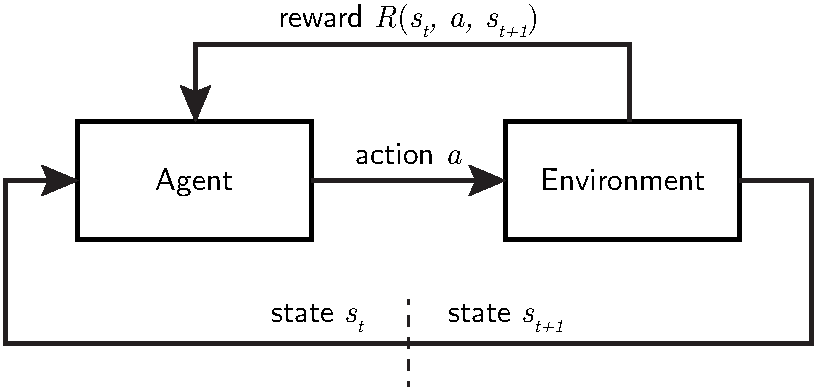
\includegraphics[width=0.6\textwidth]{mdp-2}
	\caption{Schematic representation of an \acrshort{acr:mdp} agent which repeatedly selects an action $a \in A$ based on its current state $s \in \mathcal{S}$, after which it ends up in a state $s' \in \mathcal{S}$ and receives a reward $R(s, a, s')$ accordingly.}
	\label{fig:mdp}
\end{figure}

% Reward structure
As the agent of an \acrshort{acr:mdp} aims to fulfill certain goals through the selection of actions, it requires some means of assessing which action is the best to pick.
The value measure used in \acrshortpl{acr:mdp} is defined by a mapping $R: \mathcal{S} \times A \times \mathcal{S} \mapsto \mathbb{R}$ from states and actions to real-valued \textit{rewards} (in case of added value) and/or \textit{costs} (in case of lost value).
Due to the uncertainty in the modeled system, typically the agent uses the \acrshort{acr:mdp}'s transition distribution (defined by transition function $\delta$) to compute expected values, and accordingly selects actions that maximize this quantity.
Putting these components together results in \autoref{def:mdp} below.

% Formal definition
%Putting all of these components together, an \acrshort{acr:mdp} can be defined as a 5-tuple, $\mathcal{M} = (\mathcal{S}, s_0, A, \delta, R)$ with $\mathcal{S}$ as state space, $s_0 \in \mathcal{S}$ as the initial state, $A$ as finite set of possible actions, $\delta$ as probabilistic transition function and $R$ as reward function.
\begin{definition}
	\label{def:mdp}
	A \textit{\acrfull{acr:mdp}} is a 5-tuple $(\mathcal{S}, s_0, A, \delta, R)$, where $\mathcal{S}$ is a state space, $s_0 \in \mathcal{S}$ an initial state, $A = \{a_1, \ldots, a_m\}$ a finite set of actions to choose from, $\delta: \mathcal{S} \times A \times \mathcal{S} \mapsto [0, 1]$ a probabilistic transition function and $R: \mathcal{S} \times A \times \mathcal{S} \mapsto \mathbb{R}$ a reward function.
\end{definition}

In \autoref{fig:mdp} a schematic representation is shown of how an agent operates in an environment under the \acrshort{acr:mdp} framework.
That is, in each decision epoch, the agent selects an action $a \in A$ and executes it in the environment causing a state transition from the current state $s \in \mathcal{S}$ to some state $s' \in \mathcal{S}$ where-after a reward $R(s, a, s')$ is received accordingly.

% Policies
In the context of \acrshort{acr:dtp}, \acrshortpl{acr:mdp} are used to find an optimal course of action, often referred to as a plan or \textit{policy} $\pi: \mathcal{S} \mapsto A$.
For an \acrshort{acr:mdp} the optimal policy typically means the policy that when applied by an agent, maximizes the expected value.
However, one can also choose to express goals in alternative ways which do not require the specification of a reward function.
An example of this can be seen in \cite{bhatia2010sampling, lacerda2015optimal}, which replace the reward function of the classic \acrshort{acr:mdp} framework by a (co-safe) Linear Temporal Logic (LTL) formula to be satisfied.

\subsubsection{Partially Observable MDPs}
\label{sec:pomdps}

% Observations: .. POMDP
% Reward Models and Value Functions

An extension of the traditional \acrshort{acr:mdp} models, are the \acrfull{acr:pomdp} models which account for uncertainty in the observations that are made by agents.
That is, while an \acrshort{acr:mdp} is used to model systems that are fully observable, in a \acrshort{acr:pomdp} the states are not observable and can only be inferred from the observations that are perceived.
In other words, we can intuitively view a \acrshort{acr:pomdp} as the combination of a \acrshort{acr:hmm} and an \acrshort{acr:mdp}.
As such a \acrshort{acr:pomdp} can be defined as in \autoref{def:pomdp} below.

\begin{definition}
	\label{def:pomdp}
	A \textit{\acrfull{acr:pomdp}} is a 7-tuple $(\mathcal{S}, s_0, A, \delta, \mathcal{O}, \Omega, R)$ where $\mathcal{S}$ is a state space, $s_0 \in \mathcal{S}$ an initial state, $A = \{a_1, \ldots, a_m\}$ a finite set of actions to choose from, $\delta: \mathcal{S} \times A \times \mathcal{S} \mapsto [0, 1]$ a probabilistic transition function, $\mathcal{O}$ an observation space, $\Omega: \mathcal{S}\times A \mapsto \mathcal{O}$ an emission or observation probability function and $R: \mathcal{S} \times A \times \mathcal{S} \mapsto \mathbb{R}$ a reward function.
\end{definition}

%As such, a \acrshort{acr:pomdp} can be defined as a 7-tuple $\mathcal{M} = (\mathcal{S}, s_0, A, \delta, \mathcal{O}, \Omega, R)$ with $\mathcal{S}$ as state space, $s_0 \in \mathcal{S}$ as the initial state, $A$ as finite set of possible actions, $\delta$ the transition function, $\mathcal{O}$ the observation space, $\Omega$ an emission or observation probability function and $R$ as reward function.
As the true state of a \acrshort{acr:pomdp} is unknown, the transition function $\delta$ is defined over beliefs of states, and accordingly a policy $\pi$ maps beliefs to actions.
The observation function $\Omega$ defines the probability of observations from state-action pairs in the \acrshort{acr:pomdp} and is used to iteratively update the belief state of an agent.

%TODO Check if we can put this somewhere else, or should just leave it out
%\subsubsection{Other Markov Models and Related State-Space Models}
%\label{subsec:other-markov-models}
%Apart from the discrete-state Markov Models that were discussed in this section, there exist numerous other types of Markov Models and closely related State-Space Models (SMMs), including among others the following:%, including continuous-state Markov Models (e.g., Linear Dynamical Systems with a Gaussian state-space \cite{Minka1999,barberBRML2012}) and other specialized variations. 

%\begin{description}
%	\item[Factored Markov Decision Process (FMDP)] An extension of the MDP model that allows for compact representation of states, transitions and rewards \cite{Degris2010}. In many real-life domains especially the state-space grows exponentially with the number of variables. Therefore FMDPs can be used to exponentially reduce the representation by means of a dynamic Bayesian network. The main drawback, however, is that finding the best policy becomes an NP-hard problem.
%	\item[Multi-Agent \acrshort{acr:mdp} (MMDP)] An \acrshort{acr:mdp} model for systems that involve multiple decision makers. In this model each agent chooses an individual action with the goal of optimizing a joint reward. Other variations involving multiple agents are Decentralized \acrshortpl{acr:mdp} (Dec-MDPs) and \acrshortpl{acr:pomdp} (Dec-POMDPs), which differ from MMDPs in that the agents can only approximate the global state of the process by their own (local) observations \cite{Melo20111757}.
%	%\item[Variable-order Markov Model (VOM)] To be determined 
%	\item[Linear Dynamical System (LDS)] A continuous-state State-Space Model with linear dynamics, Gaussian state space and the assumption of hidden variables as in \acrshortpl{acr:hmm} \cite{Minka1999, barberBRML2012, Ghahramani2000}.
%\end{description}
% TODO Extend each with sentence to explain the need for these models

%As the remaining chapters only consider systems and processes that are modeled using discrete-state Markov Models, these variations will not be further discussed in more detail.

\newpage

\subsection{Learning Markov Models}
\label{sec:learning-markov-models}

%\paragraph*{Fitting Markov Chains}
There exist efficient methods for fitting a discrete stationary first-order Markov Chain provided a dataset describing the evolution of a stochastic process either by applying likelihood maximization (e.g., see \cite{bacciu2015probabilistic, barberBRML2012, lee1968maximum, teodorescu2009maximum}) or Bayesian inference (e.g., see \cite{barberBRML2012, lee1968maximum, minka2003bayesian}).
These methods estimate the transition distribution to fit a Markov Chain on a collected sequence of time-ordered states.
One may obtain such a sequence by applying clustering algorithms such as $k$-means on the dataset and accordingly make predictions for each of the entries.

The first-mentioned approach of likelihood maximization, works by estimating the transition probabilities by counting the observed transitions in the state sequence.
That is, if we let $n_{ij}$ denote the number of observed transitions from state $s_j$ to state $s_i$, then the maximum-likelihood estimation of the corresponding transition probability is
\begin{equation}
p(q_{t+1} = s_i\vert q_t = s_j) = \frac{n_{ij}}{\sum_j n_{ij}}
\end{equation}

The second-mentioned approach of Bayesian inference is more suitable for many real-life problems for which state sequences are incomplete, i.e. states are recorded only for certain stages, meaning there might be gaps in-between.
This type of approach aims to make an estimation of the transition probabilities by adopting a prior for the transition matrix $\mat{A}$, a convenient choice being a factorized prior from the product of $n$ independent \textit{Dirichlet} distributions, one for each row $\mat{A}_j$, such that:
\begin{equation}
p(\mat{A}) = \prod_{j} \text{Dir}(\mat{A}_j \vert \alpha_j)
\end{equation}
parametrized by a vector $\arr{\alpha}$ with $\alpha_j > 0$ \cite{pasanisi2012estimating,barberBRML2012}.

Due to the close nature of \acrshortpl{acr:mdp} these approaches can be applied almost directly to learn transition probabilities of discrete-state \acrshortpl{acr:mdp}, although more data will be required due to the addition of actions.
To learn partially observable models, on the other hand, one requires algorithms that work with a set of observations and estimate emission probabilities.
For this thesis, however, we limit ourselves to learning fully observable \acrshortpl{acr:mdp}, but review these algorithms for learning \acrshortpl{acr:hmm} and \acrshortpl{acr:pomdp} in \autoref{sec:learning-probabilistic-models}.

\subsection{Learning Optimal Policies}
\label{sec:planning}

In \acrshort{acr:sdm} problems, typically the aim is to determine a policy that maximizes the total expected value.
In algorithmic planning techniques a probabilistic model of the environment, which includes estimates of the transition probabilities and rewards, is used to obtain an optimal policy by exploring its state space towards a goal.
On the other hand, in \acrfull{acr:rl} the optimal policy is learned while interacting with the environment and it is applied when one does not know the transition probabilities and rewards for the system in advance.
Both techniques have in common that they iteratively update estimations of a value function to derive a policy.
The main difference though is that in planning this progress is carried out based on simulated experience from a model, while in learning techniques this is based on real experience from executing agents in an environment \cite{sutton1998reinforcement}.
All by all, planning and \acrshort{acr:rl} are closely related and various ideas can be exchanged between the two.

In this section, various solutions that utilize the \acrshort{acr:mdp} framework for obtaining optimal policies are discussed.
First off, the most common \acrshort{acr:dtp} algorithms for (discrete) \acrshortpl{acr:mdp} are shown and explained.
This is followed by a discussion of the most used algorithms in \acrshort{acr:rl}.
%So, even when considering the differences, various solutions can be exchanged between planning and \acrshort{acr:rl} techniques.

%In this section the various approaches for finding optimal policies are discussed, where the planning techniques are discussed in \autoref{subsec:model-based-planning}, and \acrshort{acr:rl} techniques are discussed in \autoref{subsec:reinforcement-learning}.

% Sutton and Barto (1998/2012) describe two approaches for rl solutions when the transition and reward functions are not known	(Learning the Structure of Factored Markov Decision Processes inReinforcement Learning Problems)
% See chapter 8.2, show an adapted version of the figure and explain advantages and disadvantages
% Explain the difference between planning and learning



\subsubsection{Model-Based Planning Techniques}
\label{sec:model-based-planning}

\begin{figure}[!t]
	\centering
	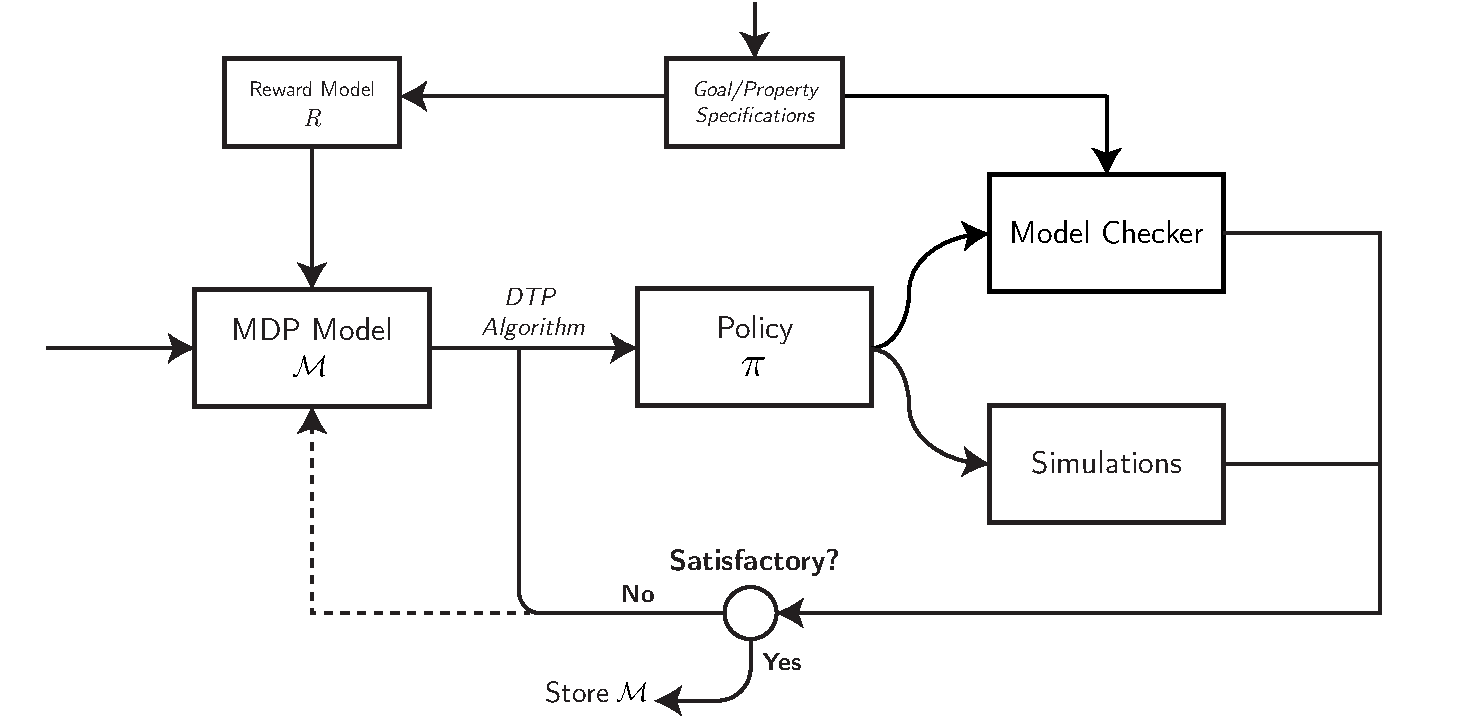
\includegraphics[width=\textwidth]{mdp-planning-diagram-v32-cropped}
	\caption{Block diagram of the generic routine employed in model-based MDP planning techniques.}
	\label{fig:model-based-routine}
\end{figure}

In \acrshort{acr:dtp} the algorithms compute their plans or policies based on a probabilistic model of the environment.
Most common is to prepare an \acrshort{acr:mdp} and apply exact dynamic programming solutions to compute an optimal policy for that model.
The routine that is typically followed in \acrshort{acr:mdp} planning is depicted in \autoref{fig:model-based-routine}.
The state space, transition function and action space are usually handcrafted, based on expertise or trial and error.
The goal that should be fulfilled is translated into a reward model, mapping positive highly-valued rewards to desirable states and low rewards/costs to states that are not desirable or need to be avoided.
These parts together form the \acrshort{acr:mdp} which is fed to a planning algorithm, often referred to as an \textit{\acrshort{acr:mdp} solver}.
From this solver, a policy $\pi$ is obtained, which is usually evaluated through simulations or automated model checking tools to check if the policy will satisfy the set of goals.
%usually evaluated by applying it in one or more simulations, rather than using it in a real-world environment.
%Another option is to make use of automated model checking tools which can verify whether the policy will satisfy the set goals. %TODO Add citation to book about model checking from APS and Bruno?
After evaluating the current policy, one may choose to stick with the current policy or adjust the parameter settings of the solver or \acrshort{acr:mdp} model and obtain a new policy.

%There are several options for the \acrshort{acr:mdp} solver, which compute an optimal policy by maximization of the expected value to be obtained.
%In the remainder of this section various of these planning algorithms for \acrshortpl{acr:mdp} are discussed and evaluated.

\paragraph{Value Iteration}
\label{sec:value-iteration}

\begin{algorithm}[!t]
	\caption{Value iteration}
	\label{alg:vi}
	\begin{algorithmic}[1]
		\Require{MDP $\mathcal{M} = (\mathcal{S}, s_0, A, \delta, R)$, discount factor $\gamma \in (0, 1)$, threshold $\xi > 0$}
		\Ensure{Optimal policy $\arr{\pi}^*: \mathcal{S} \mapsto A$}
		\State{Initialize $V_t: \mathcal{S} \mapsto \mathbb{R}$ arbitrarily for $t = 0$}
		\State $t \gets 0$
		\Repeat
		\State $t \gets t + 1$
		\ForAll{$s \in \mathcal{S}$}
		\State{$V_t(s) \gets \max_{a \in A} \left[\sum_{s' \in \mathcal{S}} \delta(s, a, s') \cdot \left[R(s, a, s') + \gamma \cdot V_{t-1}(s')\right]\right]$}
		\EndFor
		\Until{$\forall s \in \mathcal{S}: \lvert V_t(s) - V_{t-1}(s) \rvert \leq \xi$}
		\ForAll{$s \in \mathcal{S}$}
		\State $\arr{\pi}^*(s) \gets \text{arg max}_{a \in A} \left[\sum_{s' \in \mathcal{S}} \delta(s, a, s') \cdot \left[R(s, a, s') + \gamma \cdot V_{t}(s')\right]\right]$
		\EndFor
		\State\Return $\arr{\pi}^*$
	\end{algorithmic}
\end{algorithm}

The most well-known algorithm for obtaining optimal policies from \acrshortpl{acr:mdp} is \textit{\acrfull{acr:vi}}, which is a synchronous dynamic programming solution which iteratively updates a value function $V: \mathcal{S} \mapsto \mathbb{R}$ until convergence, given an \acrshort{acr:mdp} model $\mathcal{M} = (\mathcal{S}, s_0, A, \delta, R)$.
The updates are performed through so-called \textit{Bellman backups} based on the following Bellman equation:
\begin{align}
V^*(s) &= max_{a \in A} \left[\sum_{s' \in \mathcal{S}} P(s' \vert s, a) \cdot \left[R(s, a, s') + \gamma \cdot V^*_{t}(s')\right]\right]	&\forall s \in \mathcal{S}
\end{align}
where $\gamma \in (0,1)$ is a discount factor which expresses the magnitude of preference of short-term solutions over long-term solutions. That is, the smaller the factor $\gamma$, the more important it is that goals are reached in as few steps as possible.

In \autoref{alg:vi}, it is shown how the \acrshort{acr:vi} algorithm can be used to obtain optimal policies for an MDP (based on the formulation in \cite{poole2010artificial}).
Intuitively, \acrshort{acr:vi} can be viewed as estimating the values starting from the goal-rewards and working backwards.
The initial values of the value function, stored in $V_0$, can be arbitrarily initialized, but to achieve faster convergence it is customary to do the initialization based on a rough estimation of $V^*$.
In every iteration, the estimates of the value function are updated by the backup operations based on the value in previous operations.
After a finite number of iterations the algorithm will converge (as is shown in \cite{puterman2014markov}) and after that point $V(s)$ gives us the maximum to be expected sum of rewards starting from a state $s \in \mathcal{S}$.
As can be seen in \autoref{alg:vi}, convergence is reached as soon as the change in value gets below a given threshold $\xi > 0$.
After such convergence has been reached, the policy can be defined by selecting the action $a \in A$ for each state $s \in \mathcal{S}$ that is most likely to maximize the collected rewards based on the value of $V_t(s)$.
All by all, the algorithm works well when the state space is relatively small, but for large state spaces more storage is required and it may take longer to reach convergence.

Note that an alternative formulation of the \acrshort{acr:vi} algorithm can be given that makes use of a $Q$-table instead of a value function $V$ \cite{singh2000convergence}.
In this formulation the entries $Q(s, a)$ are updated in each iteration for each state-action pair.
The optimal policy can then be obtained directly by selecting the action with the maximum value in the $Q$-table for each action, though it requires more storage compared to a value function.

\paragraph{Asynchronous Value Iteration}
\label{sec:gs-value-iteration}

An adaptation of the traditional \acrshort{acr:vi} algorithm is \textit{asynchronous \acrshort{acr:vi}}, which is an asynchronous dynamic programming solution.
Almost all of the steps in asynchronous \acrshort{acr:vi} are the same except that rather than updating the value function $V: \mathcal{S} \mapsto \mathbb{R}$ for each state in each iteration, the function is updated only for a single state in each iteration in no particular order (or even randomized).
In the case of a fixed ordering, this algorithm is usually referred to as \textit{Gauss-Seidel \acrshort{acr:vi}}.
Compared to the traditional \acrshort{acr:vi} algorithm, the asynchronous adaptation requires less space and converges faster, especially when updates occur more often for most relevant states and the update ordering is adjusted carefully.

\textit{\acrfull{acr:rtdp}} \cite{barto1995learning} is a family of asynchronous \acrshort{acr:vi} algorithms which aim to find policies by performing updates and concurrently controlling the \acrshort{acr:mdp} (based on the policy corresponding to the latest estimate of the value function).
Opposed to traditional \acrshort{acr:vi}, where solving \acrshortpl{acr:mdp} with large state spaces is infeasible, RTDP algorithms often converge without examining all states.

% TODO POMDP Adaptation of Value Iteration See AI: A Modern Approach + Probabilistic Robotics

\paragraph{Policy Iteration}
\label{sec:policy-iteration}

\begin{algorithm}[!t]
	\caption{Policy iteration}
	\label{alg:pi}
	\begin{algorithmic}[1]
		\Require{MDP $\mathcal{M} = (\mathcal{S}, s_0, A, \delta, R)$, discount factor $\gamma \in (0, 1)$}
		\Ensure{Optimal policy $\arr{\pi}^*: \mathcal{S} \mapsto A$}
		\State{Initialize $\arr{\pi}_0$}
		\State $t \gets 0$
		\Repeat
		\State Solve $\forall s \in \mathcal{S}$: $V_{\arr{\pi}_{t}}(s) \gets \sum_{s' \in \mathcal{S}} \delta(s, \arr{\pi}_t(s), s') \cdot \left[R(s, \arr{\pi}_t(s), s') + \gamma \cdot V_{\arr{\pi}_{t}}(s')\right]$
		\State $t \gets t + 1$
		\ForAll{$s \in \mathcal{S}$}
		\State $\arr{\pi}_t(s) \gets \argmax_{a \in A} \left[\sum_{s' \in \mathcal{S}} \delta(s, a, s') \cdot \left[R(s, a, s') + \gamma \cdot V_{\arr{\pi}_{t - 1}}(s')\right]\right]$
		\EndFor
		\Until{$\arr{\pi}_{t} = \arr{\pi}_{t - 1}$}
		\State\Return $\arr{\pi}_t$
	\end{algorithmic}
\end{algorithm}

Another algorithm that is widely applied for obtaining policies from \acrshortpl{acr:mdp} is known as \textit{\acrfull{acr:pi}}. As shown in \autoref{alg:pi} \acrshort{acr:pi} starts off with an initial policy vector $\arr{\pi}_0$ which may be arbitrarily initialized, but preferably by an approximation of an optimal policy for the input \acrshort{acr:mdp} $\mathcal{M} = (\mathcal{S}, s_0, A, \delta, R)$ to achieve faster convergence.
Then, in each iteration, first the value for each state is computed based on the latest policy $\arr{\pi}_t$, which comes down to solving a set of linear equations.
Solving this set of linear equations can be done by linear programming in (at most) $O(\lvert\mathcal{S}\rvert^3)$ time \cite{littman1995complexity}. 
An alternative approach, known as \textit{modified policy iteration}, is to solve these by applying a simplified form of value iteration in which the actions to select are already known for each state from the policy (i.e., $\arr{\pi}_t(s)$ for each $s \in \mathcal{S}$).
This step which is known as \textit{policy evaluation} is followed by a \textit{policy improvement} step in which the policy is greedily updated based on the latest value function $V_{\arr{\pi}}$.
This process is repeated until no improvements are possible and the policy stops changing.

Compared to \acrshort{acr:vi} the algorithm always converges in a finite number of iterations. However, solving the set of linear equations in each iteration is a more time-costly operation, especially for large state spaces.
That is, in \acrshort{acr:vi} each iteration takes $O(\lvert\mathcal{S}\rvert^2\cdot\lvert A\rvert)$ time, although one must note that the number of iterations is not finite, while \acrshort{acr:pi} finds an optimum in a finite number.

\paragraph{Backwards Induction}
\label{sec:backwards-induction}

\begin{algorithm}[!t]
	\caption{Backwards induction}
	\label{alg:backwards-induction}
	\begin{algorithmic}[1]
		\Require{MDP $\mathcal{M} = (\mathcal{S}, s_0, A, \delta, R)$, horizon $h \in \mathbb{N}$}
		\Ensure{Optimal policy $\arr{\pi}^*: \mathcal{S} \mapsto A$}
		\State $t \gets h$
		\State $\forall s \in \mathcal{S}: V_h(s) \gets 0$
		\Repeat
		\State $t \gets t - 1$
		\ForAll{$s \in \mathcal{S}$}
		\State $V_t(s) \gets \max_{a \in A} \left[\sum_{s' \in \mathcal{S}} \delta(s,a,s') \cdot \left[R(s,a,s') + V_{t+1}(s')\right]\right]$
		\EndFor
		\Until{$t = 1$}
		\ForAll{$s \in \mathcal{S}$}
		\State $\arr{\pi}^*(s) \gets \argmax_{a \in A} \left[\sum_{s' \in \mathcal{S}} \delta(s,a,s') \cdot \left[R(s,a,s') + V_{1}(s')\right]\right]$
		\EndFor
		\State\Return $\arr{\pi}^*$
	\end{algorithmic}
\end{algorithm}

In the special case of a finite horizon \acrshort{acr:mdp} it is possible to obtain an optimal policy by applying \textit{backwards induction} \cite{chamie2015finite} shown in \autoref{alg:backwards-induction}.
As the name suggests the algorithm works backwards, starting from the last step $h$ and recursively using the value function of step $t + 1$ to compute that of step $t$.
Even though the algorithm works well when dealing with finite horizons, typically real world scenarios more often deal with infinite horizons for planning under uncertainty.

\paragraph{Linear Programming}
\label{sec:linear-programming}

A less frequently applied approach is that of formulating the \acrshort{acr:mdp} as a \acrfull{acr:lp} and solving it using so-called \textit{simplex} methods.
Following this approach, an \acrshort{acr:lp} formulation for an MDP $\mathcal{M} = (\mathcal{S}, s_0, A, \delta, R)$, as explained in \cite{pazis2012non}, is:

%\begin{align}
%\max_{\lambda} &\sum_{s \in \mathcal{S}}\sum_{a \in A}\sum_{s' \in \mathcal{S}} \lambda(s, a) \delta(s, a, s')R(s, a, s') &\nonumber\\
%\text{s.t.} &\sum_{a' \in A} \lambda(s', a') = \mu_0(s) + \gamma \sum_{s \in \mathcal{S}}\sum_{a \in A} \lambda(s,a)\delta(s,a,s')	&\forall s' \in \mathcal{S} \\
%&\lambda(s,a) \geq 0 &\forall s \in \mathcal{S}, \forall a \in A \nonumber
%\end{align}
\begin{align}
\min_{V} &\sum_{s' \in \mathcal{S}} \mu_0(s) \cdot V(s) &\nonumber\\
\text{s.t. } &V(s) \geq \sum_{s' \in \mathcal{S}} \delta(s, a, s') \left[R(s,a,s') + \gamma\cdot V(s')\right]	&\forall s \in \mathcal{S}, \forall a \in A
\end{align}
where $\mu_0: \mathcal{S} \mapsto [0,1]$ is a probability distribution over the states.

From the solution $V^*$ of this \acrshort{acr:lp} formulation, a policy $\arr{\pi}^*$ can be obtained by letting $\arr{\pi}^*(s) = \argmax_{a \in A} \sum_{s' \in \mathcal{S}} \delta(s, a, s') \left[R(s,a,s') + \gamma\cdot V(s')\right]$ for each state $s \in \mathcal{S}$. This primal formulation optimizes a value function $V$, but alternatively the policy can be optimized directly by considering the dual formulation (see \cite{littman1995complexity}).
Comparing \acrshort{acr:lp} solutions to the specialized \acrshort{acr:vi} and \acrshort{acr:pi} solutions, the latter typically hold more promise for efficient solutions than general-purpose \acrshort{acr:lp} algorithms, although the \acrshort{acr:lp} scale better to larger \acrshort{acr:mdp} planning problems.

\newpage

\subsubsection{Reinforcement Learning Techniques}
\label{sec:reinforcement-learning}

\acrfull{acr:rl} techniques work on real experience based on which they update the behavior of the agent which is defined by an action-selection policy. To do this they require direct interaction with the environment to obtain experience and update value function estimations accordingly during execution.
Although most planning algorithms cannot be used for learning problems, learning algorithms can be used for planning problems as they can make use of simulated experience.
There are several techniques that exist, of which the most common ones are discussed in the remainder of this section.

\paragraph{Q-Learning}
\label{sec:q-learning}

Q-Learning \cite{dayan1992q, sutton1998reinforcement} is a model-free reinforcement learning technique which discovers an action-selection policy by learning estimates of the optimal Q-values of an \acrshort{acr:mdp}.
The technique starts off with a Q-table $Q$, which is arbitrarily initialized, containing the Q-values $Q(s,a)$ for each state-action pair $(s,a)$.
At each point in time the agent for which the Q-Learning technique is applied is assumed to be in a certain state $s$ and chooses a next action $a$ to execute based on the current Q-value estimates.
After executing an action the agent ends up in a new state $s'$ and observes a certain reward $r$.
The Q-table is then updated accordingly based on the following update rule:
\[
Q(s, a) = Q(s, a) + \alpha \Big[r + \gamma \max_{a'} Q(s',a') - Q(s, a)\Big]
\]
where $\alpha \in (0,1)$ is the learning rate and $\gamma \in (0, 1)$ the discount factor.
The learning rate expresses the rate at which newly acquired information overrides the old information in the Q-table.
Over time the estimates in the Q-table will improve such that the revenue is maximized.
A near-optimal policy can then be constructed by selecting the action with the highest Q-value from the Q-table for each state.

% 
% Also note that it can be used for planning

\paragraph{SARSA}
\label{sec:sarsa}

\begin{algorithm}[!t]
	\caption{SARSA}
	\label{alg:sarsa}
	\begin{algorithmic}[1]
		\Require{State space $\mathcal{S}$, action space $A$, learning rate $\alpha$, discount factor $\gamma$}
		\Ensure{Optimal policy $\arr{\pi}^*: \mathcal{S} \mapsto A$}
		\State Initialize $Q: \mathcal{S} \times A \mapsto \mathbb{R}$ arbitrarily
		\Repeat
		\State Pick $s \in \mathcal{S}$ arbitrarily
		\State $a \gets \pi[s]$ \Comment{$\pi$ is the policy derived from $Q$}
		\Repeat
		\State Perform $a$ and observe $r, s'$
		\State $a' \gets \pi[s']$
		\State $Q(s,a) \gets Q(s,a) + \alpha \Big[r + \gamma Q(s', a') - Q(s, a)\Big]$
		\State Update $\pi$ based on $Q$
		\State $s \gets s'$
		\State $a \gets a'$
		\Until{$s$ is terminal}
		\Until{$Q$ converged}
		\State\Return $\arr{\pi}^*$
	\end{algorithmic}
\end{algorithm}

SARSA \cite{sutton1998reinforcement} is another model-free \acrshort{acr:rl} algorithm which is similar to Q-Learning.
While Q-Learning is an off-policy method which learns the value of the optimal policy, SARSA is an on-policy method which learns the value of the policy it currently follows in order to iteratively improve this policy.
In each iteration, it simulates the action yielded by its policy and observes the reward and next state.
Accordingly the $Q$-table is updated based on these observations as shown in \autoref{alg:sarsa}, which repeats itself with the observed $s'$ and action $a'$ imposed by the policy $\pi$ that is derived from $Q$.



\newpage

\section{Bayesian Optimization}
\label{sec:bayesian-optimization}

This section elaborates upon a method known as \acrfull{acr:bo}, which is used to automate the process of optimizing the parameters of an unknown objective.
First \autoref{sec:bayesian-optimization-problem} introduces the optimization tasks this method is aimed at and how these are relevant to \acrshort{acr:sdm} problems.
Subsequently, in \autoref{sec:bayesian-optimization-algorithm} the optimization method is formally described.
In \autoref{sec:bayesian-optimization-prior-acquisition} the configurable parts of the method are discussed, considering both advantages and disadvantages of available options.
Finally, in \autoref{sec:bayesian-optimization-applications} a number of applications of \acrlong{acr:bo} in the field of planning under uncertainty are discussed, serving as an overview of the method's successes in this field.

% More applications:
%https://www.cs.ox.ac.uk/people/nando.defreitas/publications/BayesOptLoop.pdf

\subsection{Problem Formulation}
\label{sec:bayesian-optimization-problem}

One of the problems that is faced in the field of optimization is that of maximizing a nonlinear, real valued \textit{objective function} $f: \mathcal{X} \mapsto \mathbb{R}$ on a domain $\mathcal{X} \subset \mathbb{R}^m$ ($m \geq 1$).
Formally, to find a global maximizer $x^\ast \in \mathcal{X}$ for which:
\begin{equation}
	x^\ast = \argmax_{x \in \mathcal{X}} f(x)
\end{equation}
In particular the problem turns out to be a common bottleneck when dealing with an objective function that is unknown and expensive to evaluate in terms of the required computational resources.
As an example, one could think of finding the hyper-parameters for a neural network which maximize the performance, where each single evaluation of a set of parameters requires one to train the neural network and assess the performance on a huge dataset.

Although this problem of optimizing expensive functions can be found in many different contexts, it is foremost a problem in sequential decision theory. 
That is, typically one can only hope to estimate objective functions of \acrshort{acr:sdm} problems in AI planning and reinforcement learning through expensive simulations \cite{Brochu2010}. 
A particularly relevant optimization problem pops up when considering the problem of learning to control systems that involve uncertainty, in which an important issue is that of faithfully modeling the uncertainty in the outcomes of actions \cite{Ghahramani2015}.
This particular problem has recently received quite some attention, posing it as a problem of learning and optimizing the parameters of a probabilistic model of the system, such as the model's transition probabilities, reward function or optimal policy \cite{Poupart2010}.

A naive approach for optimizing the objective would be to evaluate a set of (random) combinations of parameters and see which parameter-settings seem to give the best results.
This approach however, usually requires expert knowledge and might demand a large number of function evaluations that do not necessarily provide new information about the parameter-space.
The method known as \textit{\acrlong{acr:bo}}, described in \autoref{sec:bayesian-optimization-algorithm}, improves on these naive approaches by making predictions about which regions of the parameter-space are expected to give the best results and hence limiting the number of function-evaluations.

\subsection{Algorithm Description}
\label{sec:bayesian-optimization-algorithm}

\textit{\acrfull{acr:bo}} is a powerful method for finding the maximum of a typically unknown, expensive, nonlinear objective function, while aiming to minimize the number of objective function evaluations and avoiding local maxima \cite{Brochu2010}.
This method first requires one to set a prior $p(f)$ over the objective function $f$, representing the belief about the space of plausible objective functions.
Then, the algorithm starts off by gathering a small set of initial sample-observation pairs of samples $x \in \mathcal{X}$ and corresponding objective values $y = f(x) + \varepsilon$.
These pairs are then stored in a set $\mathcal{D}_{1:t} = \{(x_i, y_i) \mid i = 1 \ldots t\}$ (i.e., the \textit{evidence set}) where we let $x_i$ denote the $i$th sample and $y_i = f(x_i) + \varepsilon_i$ the corresponding $i$th observation with noise $\varepsilon_i$.
% Posterior / Surrogate Function
The algorithm then derives a posterior distribution $p(f \vert \mathcal{D}_{1:t})$ which, according to Bayes' Theorem, is said to be proportional to the likelihood $p(\mathcal{D}_{1:t} \vert f)$ and the prior $p(f)$ for the first $t$ gathered observations, s.t.:
\begin{equation}
	p(f \vert \mathcal{D}_{1:t}) \propto p(\mathcal{D}_{1:t} \vert f) \cdot p(f)
\end{equation}
This posterior can be viewed as an estimation of the objective function $f$, sometimes also referred to as a \textit{surrogate function}.
% It does so by applying Bayes' Theorem, which states that the posterior probability $P(M \vert E)$ of a model $M$ given evidence $E$ is proportional to the likelihood $P(E \vert M)$ of $E$ given $M$

% Acquisition function
To decide on which $x \in \mathcal{X}$ to sample and gather a new observation $f(x)$ from next, a so-called \textit{acquisition function} $u: \mathcal{X} \mapsto \mathbb{R}$ is used, which assigns a certain utility to evaluating $f$ at some particular $x \in \mathcal{X}$ given the evidence set $\mathcal{D}$ at that time.
This acquisition function should be defined such that it captures a correct balance between \textit{exploration} (to sample from areas with high uncertainty) and \textit{exploitation} (to sample from areas likely to improve on prior observations). For this reason many different classes of acquisition functions exist, which are discussed in little more detail in \autoref{sec:bayesian-optimization-prior-acquisition}.

% General Formulation Algorithm

\begin{algorithm}[!t]
	\caption{\acrlong{acr:bo} (General Formulation) \label{alg:bayesian-optimization}}
	\begin{algorithmic}[1]
		\Require{Domain $\mathcal{X} \subset \mathbb{R}^m (m \geq 1)$, prior $p(f)$ and acquisition function $u: \mathcal{X} \mapsto \mathbb{R}$}
		\Let{$\mathcal{D}_{1:n}$}{$\{(x_i, y_i)\}\rvert^{n}_{i=1}$} \Comment{$\mathcal{D}$ is the evidence set with $\mathcal{D}_{1:n}$ the $n$ initial sample-observation pairs}
		\For{$t \gets n + 1, n + 2, \ldots$}
			\Let{$x_t$}{$\argmax_{x \in \mathcal{X}} u(x \vert \mathcal{D}_{1:t-1})$} \Comment{Acquisition based on posterior $p(f \vert \mathcal{D}_{1:t})$}%\Comment{Retrieve the next sample}
			\Let{$y_t$}{$f(x_t) + \varepsilon_t$}  %\Comment{Record a new observation of $f$}
			\Let{$\mathcal{D}_{1:t}$}{$\mathcal{D}_{1:t-1} \cup \{(x_t, y_t)\}$} \Comment{Augment $\mathcal{D}$ with the new evidence}
			\State Update the prior $p(f)$ and posterior $p(f \vert \mathcal{D}_{1:t})$
			\State \textit{Break} when satisfactory \Comment{Stop condition defined by implementation}
		\EndFor
		\State \Return{$\argmax_{(x_i, y_i) \in \mathcal{D}} y_i$}
	\end{algorithmic}
\end{algorithm}

The general formulation of the \acrshort{acr:bo} framework is presented in \autoref{alg:bayesian-optimization}.
For an implementation of the algorithm still three components need to be defined, which are the domain $\mathcal{X}$ of $f$, the prior over $f$, and last of all the acquisition function $u$.

\subsection{Choice of Prior and Acquisition Function}
\label{sec:bayesian-optimization-prior-acquisition}
In order to apply \acrlong{acr:bo} there are two major choices that need to be made, which are those of the prior distribution over the objective and the acquisition function. In this section the different options and corresponding considerations that need to be made for these two components are elaborated upon.

\subsubsection*{Prior Distributions}
\label{sec:bayesian-optimization-prior}
In \acrlong{acr:bo} the most common choice for the prior distribution is a \acrfull{acr:gp}, which is typically well-suited as it accounts for the uncertainty associated with each prediction.
Another important aspect that makes a \acrshort{acr:gp} a convenient choice for the prior distribution is that it induces a posterior distribution over the objective function that is analytically tractable.
Intuitively a \acrshort{acr:gp} can be viewed as a prior which assumes that similar inputs result in similar outputs.
For an objective function $f$, the \acrshort{acr:gp} defines a Gaussian probability distribution over $f(x)$ for each $x$, so that a \acrshort{acr:gp} can be expressed as a probability distribution over functions:
\begin{equation}
	P(f(x) \vert x) = \mathcal{N}(\mu(x), \sigma^2(x))
\end{equation}
where $\mathcal{N}$ denotes a normal distribution, while $\mu$ and $\sigma$ denote mean and standard deviation respectively.
By this definition, a \acrshort{acr:gp} can be viewed as a function that returns the mean and variance of a normal distribution over the possible values of $f$ at $x$. A \acrshort{acr:gp} as prior over an objective function $f$ is typically denoted as: 
\begin{equation}
\label{eq:gp}
f \sim GP(m(\cdot), K(\cdot, \cdot))
\end{equation}
so that the \acrshort{acr:gp} is completely specified by a mean function $m$ and a \textit{kernel} function $K$ defining the covariance.
The mean function $\mu$ is typically initialized by a constant mean, usually zero, due to the assumption that all points in the parameter space are equally likely and because the conditional mean can still be flexibly specified by the kernel function $K$ \cite{kawaguchi2015bayesian}.
\newpage
The choice of the kernel or covariance function of the \acrshort{acr:gp} determines the smoothness of the estimations on the performance and confidence intervals of unexplored samples in the parameter space.
According to the various literature in the field of \acrlong{acr:bo} the most common kernels are said to be the \textit{squared exponential} (also known as \textit{radial basis function (RBF)} or Gaussian) kernel and Mat\'ern kernel.
However, the squared exponential kernel turns out unrealistically smooth for practical applications \cite{snoek2012practical} and therefore would require properly selecting its hyper-parameters.
The Mat\'ern kernel serves as a more flexible class, where the hyper-parameters allow tweaking the distance at which there are almost no effects from previous samples and the rate at which these effects decrease, for which a reoccurring kernel appears to be an automatic relevance determination (ARD) Mat\'ern 5/2 kernel for machine learning applications \cite{snoek2012practical, kawaguchi2015bayesian}.


%\begin{itemize}
%	\item \acrfull{acr:gp}
%	\item Wiener Process
%\end{itemize}


\subsubsection*{Acquisition Functions}
\label{sec:bayesian-optimization-acquisition}
% Examples acquisition function: PMAX, IEMAX, MPI, MEI, (GP-)UCB, GP-Hedge
% TODO Introduction
The next step is defining an acquisition function which is used in the optimization process to efficiently sample observations towards the global optimum.
Typically, high utility in the acquisition functions corresponds to potentially high objective function values.
However, to avoid getting stuck in local optima, acquisition functions are defined such that a trade-off is made between exploration and exploitation.
In each iteration of \acrlong{acr:bo}, observations are sampled at the point $x \in \mathcal{X}$ where the utility is the highest.
Traditionally, the \acrfull{acr:mpi}, \acrfull{acr:mei} and \acrfull{acr:gp-ucb} functions are used for \acrlong{acr:bo}.
%This section presents an overview of the most common choices for acquisition functions used for Bayesian Optimization, together with their individual advantages and disadvantages.
In the discussion of these acquisition functions, let us define $f(x^+)$ as the `best' observation, corresponding to the sample $x^+ = \argmax_{x_i \in x_{1:t}} y_i$ when considering the first $t$ samples.
In the following overview each of these acquisition functions are defined accompanied by a discussion of their main advantages and disadvantages seen in practice.

% TODO "Best-known acquisition functions:"
\begin{description}
	\item[\acrfull{acr:mpi}] This acquisition function selects the next sample to maximize the probability of improvement, which is the sample $x \in \mathcal{X}$ so that:
	$$\argmax_{x \in \mathcal{X}} P(f(x) \geq f(x^+) + \xi)$$
	where $\xi \geq 0$ is a trade-off parameter. The higher this trade-off parameter $\xi$, the higher the preference of exploration over exploitation. Note that this means that setting $\xi = 0$ implies that the optimization purely depends on exploitation, acquiring points most likely to yield improvement. One could also choose to update $\xi$ dynamically over time.
	\begin{description}
		\item[Advantages] Intuitive acquisition function which can guarantee a minimum improvement of $\xi$ in each iteration. Considers both mean, variance and current best $f(x^+)$ of the surrogate function.
		\item[Disadvantages] Difficult to tune trade-off parameter and extremely sensitive to the choice of this parameter: a too small $\xi$ may result in an exhaustive search around a local optimum, while a too large $\xi$ results in a slow search (close to random sampling)
	\end{description}
	\item[\acrfull{acr:mei}] This acquisition function defines its utility based on the magnitude of the improvement to be expected. The function ignores the points that would lead to a decrease compared to the current best $f(x^+)$. The \acrshort{acr:mei} function selects the point $x \in \mathcal{X}$ such that:
	$$\argmax_{x \in \mathcal{X}} \mathbb{E}[\max(0, \mu_f(x) - f(x^+) - \xi)]$$
	where $\mu_f(x)$ is the posterior mean at $x$ for the objective $f$ and $\xi \geq 0$ a trade-off parameter.
	\begin{description}
		\item[Advantages] Common steps exist for properly setting $\xi$, with $\xi = 0.01$ appearing to work well in most cases according to \cite{lizotte2008practical}. Allows for non-myopic extensions \cite{Brochu2010}.
		\item[Disadvantages] Points that are likely to bring no improvement are neglected, although the chance of them resulting in actual improvement is usually small.
	\end{description}
	\item[\acrfull{acr:gp-ucb}] This acquisition function defines its utility by looking at the curve that is $\beta_t$ standard deviations above the posterior mean $\mu_f$ and samples $x \in \mathcal{X}$ such that:
	$$\argmax_{x \in \mathcal{X}} \mu_f(x) + \beta_t\sigma_f(x)$$
	where $\beta_t$ is an $\mathcal{O}(\log{t})$ exploration coefficient scheduled over time \cite{perchet2014gaussian}. This acquisition function relies on the idea of being optimistic in the face of uncertainty.
	\begin{description}
		\item[Advantages] Strong bounds exist on the cumulative regret and also guidelines exist to set $\beta_t$ to achieve optimal regret.
		\item[Disadvantages] Hyper-parameter $\beta_t$ needs to be set properly.
	\end{description}
\end{description}

In some domains, the time that is needed to evaluate the objective function depends on the region from which a point $x \in \mathcal{X}$ is sampled.
For example, when again the optimization of the hyper-parameters of neural networks is considered, one may observe that for some settings of parameters it takes a lot longer to train a model.
To account for this aspect, one could apply cost-sensitive optimization by using the \acrfull{acr:mei-ps} function
For this acquisition function that is proposed in \cite{snoek2012practical}, another \acrshort{acr:gp}-model is defined over the evaluation time of the objective function for the same domain $\mathcal{X}$.
So in each iteration the \acrshort{acr:mei-ps} function samples $x \in \mathcal{X}$ such that:
$$\argmax_{x \in \mathcal{X}} \frac{\mathbb{E}[\max(0, \mu_f(x) - f(x^+) - \xi)]}{\mu_s(x)}$$
where $\mu_s(x)$ is the posterior mean at $x$ for the timing \acrshort{acr:gp}-model.

Apart from the acquisition functions that have been discussed here, there are various other acquisition functions for specific purposes, like for example \textit{Hedge} \cite{hoffman2011portfolio} or \textit{Entropy Search} \cite{wang2016optimization} functions.

%Others possible acquisition functions that are used in Bayesian optimization are PMAX, IEMAX and GP-HEDGE. % TODO

\subsection{Applications of Bayesian Optimization to Planning Problems}
\label{sec:bayesian-optimization-applications}

% TODO Write out completely, this is just a short overview
% Most interesting applications that involve or are closely related to \acrshort{acr:dtp}:
As we consider the optimization of learning probabilistic models for planning under uncertainty in this thesis, it might be valuable to have a look at how \acrlong{acr:bo} is applied to closely related tasks for planning.
Therefore, in this section a number of applications that involve or are closely related to \acrshort{acr:dtp} are highlighted, to get an idea of the applicability of \acrlong{acr:bo} and identify the motivations for using this method.

In \cite{MartinezCantin2009}, \acrlong{acr:bo} is applied for a mobile robot that adaptively plans a path while maximizing the information it obtains from observations about its own location and the location of navigation landmarks in the environment.
The objective/cost function $C$ is parametrized by a policy-vector $\pi$ and approximations for selected samples (of robot pose and landmark locations) are made by different functions (i.e., average mean square error (AMSE), maximum a posteriori square error (MAPSE) and a largest marginal heuristic) over the belief-states of the \acrshort{acr:pomdp}.
Typically, estimating the belief-state is an expensive problem, typically carried out through SLAM algorithms in robotics.
Therefore, to minimize computational cost, a \acrlong{acr:bo} algorithm is applied with the choice of a \acrshort{acr:gp}-prior over $C$ and where new samples are acquired using an \acrshort{acr:mei} acquisition function.
Applying \acrlong{acr:bo} allows for a more cost-efficient online path planning method for optimal exploration of an environment compared to other approaches.

Another consideration for exploration of environments with stochastic dynamics is that of safety. That is, the assumption of an \acrshort{acr:mdp} being \textit{ergodic}, which is when any state is reachable from another, is impractical as systems tend to get stuck or break due to unsafe exploration. Therefore, in \cite{turchetta2016safe} a method of safe exploration is proposed that based on an initial set of states that are known a priori to be safe, iteratively identifies which nearby states are safe to visit.
This is done by making regularity assumptions on the safety feature, and by such modeling this safety feature by a \acrshort{acr:gp} prior with a Mat\'ern 5/2 kernel.
The goal of their \texttt{SAFEMDP} algorithm is to visit those states that expand the set of safe states (of which is known that a safe return route exists which is inferred from the \acrshort{acr:mdp}'s transition dynamics) as quickly as possible, so to minimize the resources required to explore the \acrshort{acr:mdp}.
Therefore, the acquisition is performed such that those states are selected that are known to be safe and comprise the highest uncertainty, so that the acquired knowledge with every sample is maximized.

Finally, another relevant example is seen in \cite{wilson2014using} in which \acrlong{acr:bo} is used to optimize policies for \acrshort{acr:rl} by exploiting generated trajectory data.
To take advantage of the obtained trajectory information in the \acrlong{acr:bo} this information is intertwined with the kernel of the \acrshort{acr:gp} prior, in such way that the induced behavior (i.e., defined by sequences of selected actions) of pairs of policies are taken into account in a behavior-based kernel (BBK).
Accordingly, given an evidence set $\mathcal{D}_{1:n} = \{(\pi_i, \eta(\pi_i), \xi_i)\}$ an (estimate) of the expected return $\eta(\pi_i)$ of policy $\pi_i$ is computed using a set of trajectories $\xi_i$.
Finally, a model-based method of \acrlong{acr:bo} is proposed as well, which learns transition probabilities and reward functions based on collected trajectory data to approximate the expected return through simulations on a probabilistic model.
To account for inaccuracies of learned models, this model-based algorithm introduces a $\beta$-term in the kernel that ensures that the model-information is neglected when it turns out to be inaccurate based on the occurrence of systematic errors.

% \cite{martinez2007active}, ... (Robot Planning and Exploration under uncertainty)

%\subsection{Extensions on Bayesian Optimization}
%\label{sec:bayesian-optimization-extensions}
%\blindtext

